\chapter{Detekcija govora mržnje}

\section{Opis zadatka}

U okviru ovog zadatka implementirana je automatska detekcija govora mržnje u tekstualnim porukama koje korisnici razmjenjuju unutar dating platformi. Zadatak je formulisan kao binarna klasifikacija: svaka poruka se svrstava u jednu od dvije klase --- \textit{govor mržnje} (label 1) ili \textit{nije govor mržnje} (label 0). Cilj je da platforma može u realnom vremenu prepoznati toksičan sadržaj i zaštititi korisnike od štetnih interakcija.

\section{Podaci}

\subsection{Pregled dataseta}

Korišćena su dva javno dostupna dataseta koja su spojena u jedinstven korpus:

\begin{itemize}
    \item \textbf{Davidson 2017} \cite{davidson2017} --- dataset od oko 25\,000 tvitova anotiranih u tri klase: \textit{hate speech}, \textit{offensive language} i \textit{neither}. Za potrebe ovog zadatka primijenjena je harmonizacija u binarni format: izvorna klasa \textit{hate speech} (0) mapirana je na label 1, dok su klase \textit{offensive} i \textit{neither} spojene u label 0. Preuzet je automatski putem skripte \texttt{src/data\_collection/download\_hate\_speech.py}.
    \item \textbf{tweet\_eval/hate} \cite{barbieri2020tweeteval} --- HuggingFace dataset koji je već u binarnom formatu (0/1), preuzet putem \texttt{datasets} biblioteke.
\end{itemize}

Nakon spajanja i uklanjanja duplikata, korpus sadrži ukupno \textbf{17\,916 primjera}, od kojih je otprilike 18\% označeno kao govor mržnje. Raspodjela klasa prikazana je u tablici~\ref{tab:hate_dist}.

\begin{table}[h]
\centering
\caption{Raspodjela klasa u kombinovanom datasetu}
\label{tab:hate_dist}
\begin{tabular}{lrr}
\hline
\textbf{Klasa} & \textbf{Broj primjera} & \textbf{Udio} \\
\hline
Nije govor mržnje (0) & 14\,717 & 82{,}1\% \\
Govor mržnje (1) & 3\,199 & 17{,}9\% \\
\hline
\end{tabular}
\end{table}

\subsection{Preprocesiranje i podjela podataka}

Preprocesiranje je implementirano u modulu \texttt{src/preprocessing/preprocess\_hate\_speech.py}. Za čišćenje teksta korišten je pipeline \texttt{clean\_for\_classification} (definisan u \texttt{src/preprocessing/text\_cleaning.py}), koji uključuje: ispravku pokvarenih Unicode karaktera, zamjenu URL-ova, e-mail adresa i telefonskih brojeva odgovarajućim tokenima (\texttt{<URL>}, \texttt{<EMAIL>}, \texttt{<PHONE>}), uklanjanje emojija, tokenizaciju, filtriranje stop-rijeci uz zadržavanje negacija i lematizaciju.

\textbf{Napomena:} TF-IDF model koristi obrađeni tekst (\texttt{text\_clean} kolona), dok Sentence-BERT model koristi originalni tekst jer transformerski tokenizator sam obavlja potrebnu normalizaciju.

Dataset je podijeljen stratificiranom metodom u omjeru \textbf{70\,\%\,/\,15\,\%\,/\,15\,\%}:

\begin{table}[h]
\centering
\caption{Veličine skupova podataka}
\label{tab:hate_splits}
\begin{tabular}{lrr}
\hline
\textbf{Skup} & \textbf{Ukupno} & \textbf{Hate (1)} \\
\hline
Train & 12\,541 & 2\,239 \\
Val   & 2\,688  & 480   \\
Test  & 2\,687  & 480   \\
\hline
\end{tabular}
\end{table}

\section{Reprezentacije teksta i modeli}

Za ovaj zadatak ispitana su dva pristupa pretvaranja teksta u numeričke vektore pogodne za klasifikaciju. U oba slučaja primijenjena je ista metoda klasifikacije --- logistička regresija s parametrom \texttt{class\_weight='balanced'} --- kako bi poređenje reprezentacija bilo ravnopravno.

\subsection{TF-IDF (klasična statistička reprezentacija)}

TF-IDF (\textit{Term Frequency -- Inverse Document Frequency}) svaki tekst pretvara u rijedak vektor težina tokena. Visoka vrijednost znači da je token karakterističan za taj tekst, ali rijedak u ostatku korpusa. Korišćeni parametri: \texttt{max\_features=20\,000}, \texttt{ngram\_range=(1,\,2)}, \texttt{min\_df=2}, \texttt{sublinear\_tf=True}.

Uključivanje bigrama (\texttt{ngram\_range=(1,\,2)}) posebno je korisno za detekciju govora mržnje jer su mnogi uvredljivi izrazi složeni od više riječi. Veći vokabular (\texttt{max\_features=20\,000}) odabran je u poređenju s detekcijom prevara zbog raznovrsnijeg Twitter rječnika. Implementacija se nalazi u \texttt{src/hate\_speech/hate\_detector.py}.

\subsection{Sentence-BERT (duboka kontekstualna reprezentacija)}

Sentence-BERT kodira cijeli tekst u gust vektor od 384 dimenzije koji predstavlja semantičko značenje teksta. Korišćen je model \texttt{all-MiniLM-L6-v2}. Za razliku od TF-IDF-a, Sentence-BERT razumije kontekst i može prepoznati semantičku sličnost između tekstova koji ne dijele isti vokabular. Enkodiranje trening skupa izvršeno je s \texttt{batch\_size=128}.

\section{Evaluacija}

\subsection{Matrice konfuzije}

Na slikama~\ref{fig:hate_cm_val_tfidf} i~\ref{fig:hate_cm_val_sbert} prikazane su matrice konfuzije na validacijskom skupu, a na slici~\ref{fig:hate_cm_test} poređenje na testnom skupu.

\begin{figure}[h]
\centering
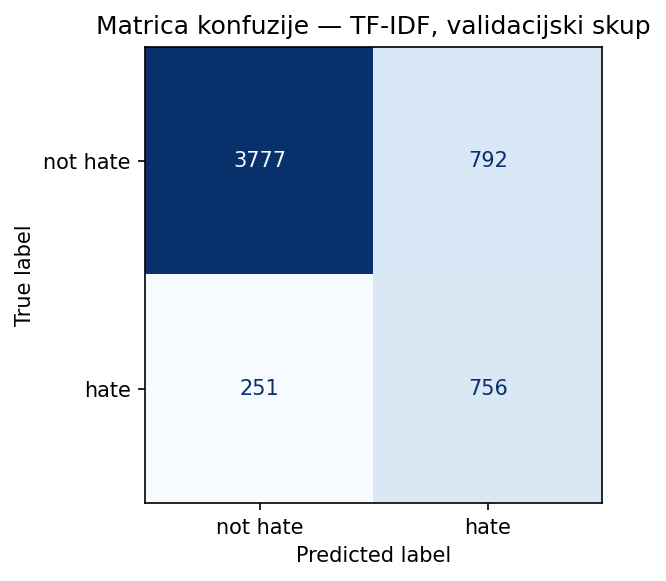
\includegraphics[width=0.55\textwidth]{figures/hate_speech/cm_tfidf_val.png}
\caption{Matrica konfuzije --- TF-IDF + LR, validacijski skup}
\label{fig:hate_cm_val_tfidf}
\end{figure}

\begin{figure}[h]
\centering
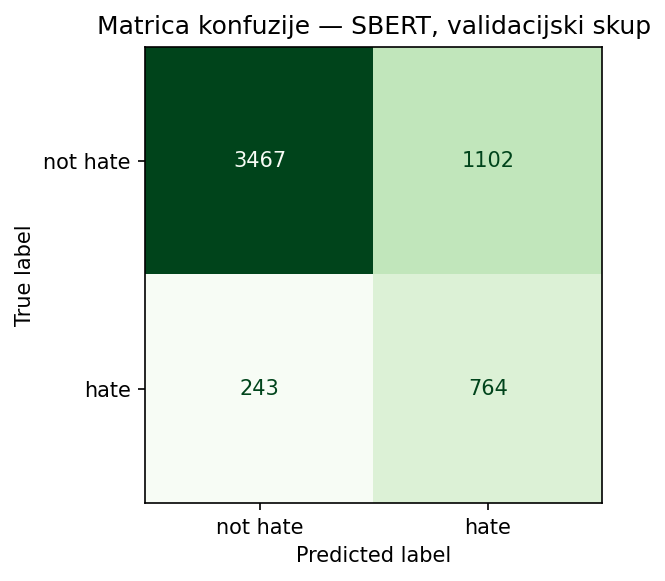
\includegraphics[width=0.55\textwidth]{figures/hate_speech/cm_sbert_val.png}
\caption{Matrica konfuzije --- Sentence-BERT + LR, validacijski skup}
\label{fig:hate_cm_val_sbert}
\end{figure}

\begin{figure}[h]
\centering
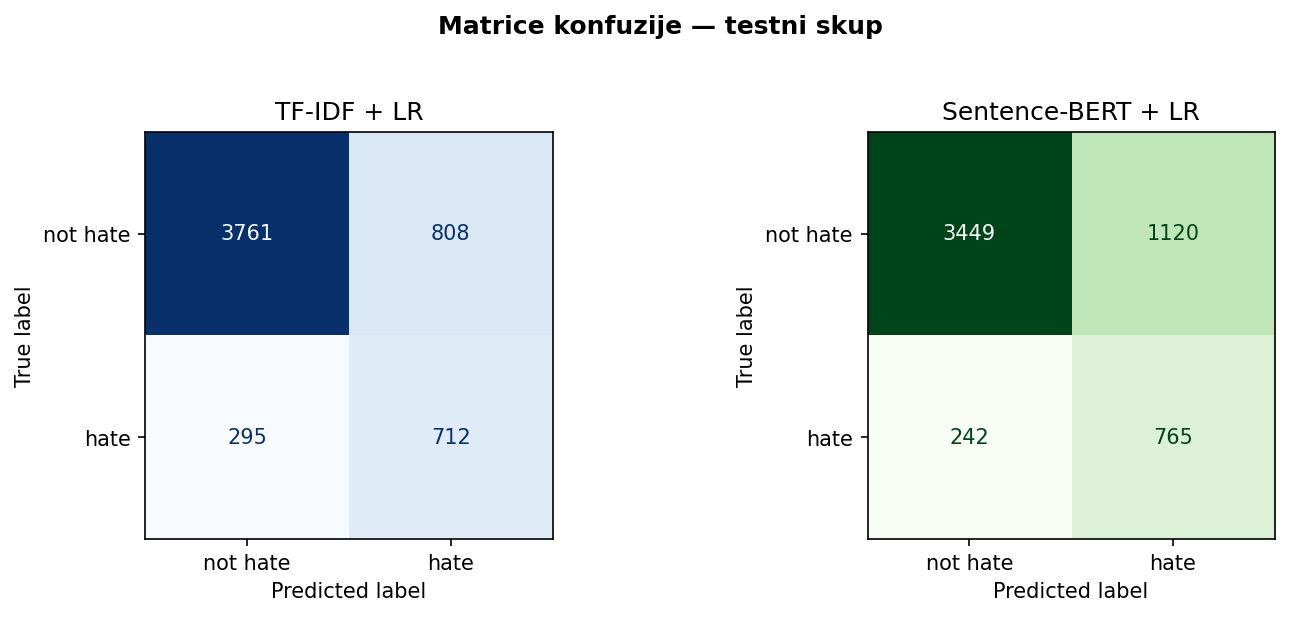
\includegraphics[width=0.9\textwidth]{figures/hate_speech/cm_test_both.png}
\caption{Matrice konfuzije na testnom skupu --- poređenje oba modela}
\label{fig:hate_cm_test}
\end{figure}

\subsection{ROC krive}

Na slici~\ref{fig:hate_roc} prikazane su ROC krive za oba modela na testnom skupu.

\begin{figure}[h]
\centering
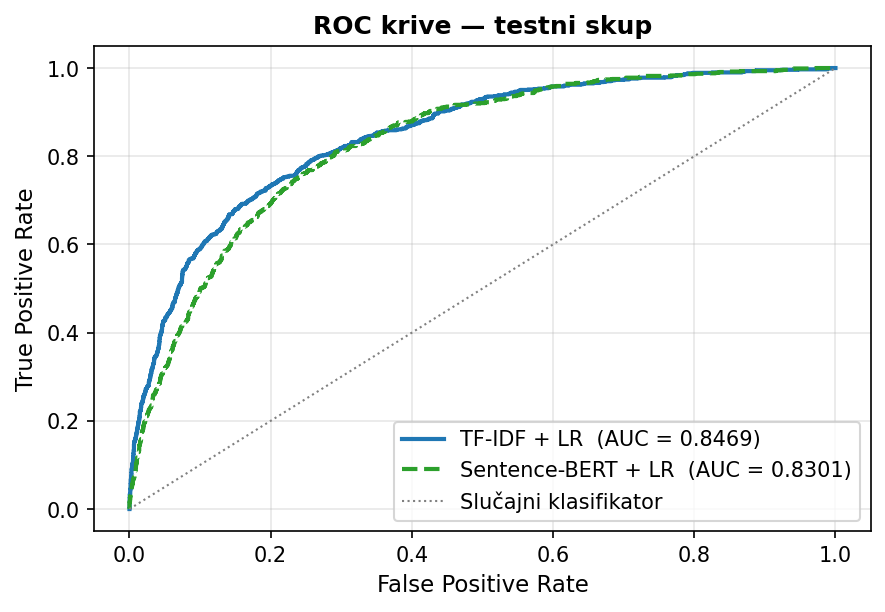
\includegraphics[width=0.7\textwidth]{figures/hate_speech/roc_test.png}
\caption{ROC krive na testnom skupu}
\label{fig:hate_roc}
\end{figure}

\subsection{Usporedba metrika}

Kompletne metrike na testnom skupu prikazane su u tablici~\ref{tab:hate_metrics} i na slici~\ref{fig:hate_bar}.

\begin{table}[h]
\centering
\caption{Metrike na testnom skupu (za klasu \textit{hate})}
\label{tab:hate_metrics}
\begin{tabular}{lrrrrr}
\hline
\textbf{Model} & \textbf{Accuracy} & \textbf{Precision} & \textbf{Recall} & \textbf{F1} & \textbf{AUC} \\
\hline
TF-IDF + LR        & 0{,}802 & 0{,}468 & 0{,}707 & 0{,}564 & 0{,}847 \\
Sentence-BERT + LR & 0{,}756 & 0{,}406 & 0{,}760 & 0{,}529 & 0{,}830 \\
\hline
\end{tabular}
\end{table}

\begin{figure}[h]
\centering
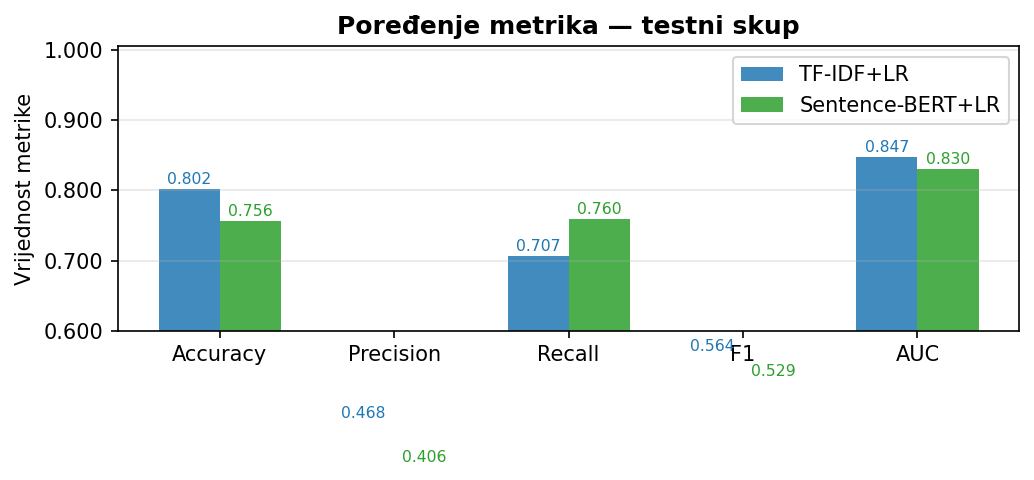
\includegraphics[width=0.8\textwidth]{figures/hate_speech/bar_metrics.png}
\caption{Poređenje metrika na testnom skupu}
\label{fig:hate_bar}
\end{figure}

\subsection{Analiza rezultata}

TF-IDF model pokazuje bolji F1 skor (0,564 vs.\ 0,529) i bolji AUC (0,847 vs.\ 0,830), kao i nešto višu preciznost. Sentence-BERT postiže nešto viši recall (0,760 vs.\ 0,707), što znači da propušta manje primjera govora mržnje, ali i pravi više lažnih uzbuna.

Oba modela bilježe nisku preciznost, što je očekivano za zadatak detekcije govora mržnje. Govor mržnje dijeli velik dio vokabulara s legitimnim, ali izraženim kritičkim govorom --- bez dublje analize konteksta, pragmatičnih i kulturnih nijansi, klasifikator nije u stanju uvijek precizno razlikovati te kategorije. Dobijene vrijednosti F1~$\approx$~0,56 konzistentne su s rezultatima objavljenim u literaturi za slične skupove podataka i metodologije \cite{davidson2017}.

\subsection{Podešavanje praga odluke}

Podrazumijevani prag klasifikacije od 0,50 nije nužno optimalan za zadatke s neravnomjernom raspodjelom klasa. Kompromis između preciznosti i odziva može se kontrolisati promjenom praga: viši prag smanjuje lažne uzbune (legitimni sadržaj pogrešno flagovan), dok niži prag povećava osjetljivost modela na hate sadržaj. Analiza krive F1 u ovisnosti o pragu na validacijskom skupu prikazana je u bilježnici \texttt{notebooks/03\_hate\_speech.ipynb}. Streamlit aplikacija implementira interaktivno podešavanje praga za svaki model odvojeno, čime se demonstrira ovaj efekt u realnom vremenu.

\section{Opis implementacije}

Implementacija je organizovana na sljedeći način:

\begin{itemize}
    \item \texttt{src/hate\_speech/hate\_detector.py} --- klasa \texttt{HateDetector} koja enkapsulira oba modela, metode za treniranje (\texttt{fit\_tfidf}, \texttt{fit\_sbert}) i predikciju (\texttt{predict\_tfidf(text, threshold)}, \texttt{predict\_sbert(text, threshold)}), te metodu za ekstrakciju najvažnijih TF-IDF tokena (\texttt{tfidf\_top\_features}). Metode predikcije prihvataju parametar \texttt{threshold} (podrazumijevana vrijednost 0,50) koji kontroliše granicu odluke između klasa.
    \item \texttt{src/ui/hate\_speech\_app.py} --- Streamlit aplikacija za interaktivnu demonstraciju. Pokreće se komandom \texttt{streamlit run src/ui/hate\_speech\_app.py}. Rezultati su prikazani u tabovima za svaki model, s vizualizacijom praga na grafikonu vjerovatnoće i interaktivnim klizačima praga u bočnoj traci. Modeli se kešuju korištenjem \texttt{@st.cache\_resource} dekoratora.
    \item \texttt{notebooks/03\_hate\_speech.ipynb} --- Jupyter bilježnica s kompletnom analizom: učitavanje podataka, treniranje oba modela, evaluacija na validacijskom i testnom skupu, vizualizacije i zaključci.
\end{itemize}

\section{Zaključak}

Implementirana su dva pristupa detekciji govora mržnje. TF-IDF s logističkom regresijom postiže nešto bolji ukupni F1 i AUC na testnom skupu, što upućuje na to da karakteristični vokabular igra ključnu ulogu u ovom datasetu. Sentence-BERT postiže viši recall, što ga čini pogodnijim u scenarijima gdje je propuštanje slučajeva govora mržnje skuplje od lažnih uzbuna.

Prirodna nadogradnja ove implementacije bila bi fino podešavanje (\textit{fine-tuning}) domenski specifičnog modela poput HateBERT-a \cite{caselli2020hatebert} na kombinovanom skupu podataka, što bi vjerovatno rezultiralo značajnim povećanjem F1 skora (na vrijednosti između 0,70 i 0,80 prema literaturnim referencama).
